%\documentclass[a4paper]{article}
\documentclass[preprint]{elsarticle}
%\usepackage[affil-it]{authblk}
%\setcounter{Maxaffil}{30}
\usepackage{footmisc}
%\usepackage{fnpct}
\makeatletter
\let\@fnsymbol\@alph
\makeatother
\usepackage[english]{babel}
\usepackage[utf8]{inputenc}
\usepackage{fancyhdr}
\setlength{\headheight}{100.0pt}
\usepackage{amsmath}
\usepackage{amssymb}
\usepackage{upgreek}
\usepackage{graphicx}
\usepackage{endnotes}
\usepackage{float}
\usepackage{caption}
\usepackage{subcaption}
\usepackage[colorinlistoftodos]{todonotes}
\usepackage{url}
\usepackage{lineno}
\usepackage{appendix}
\usepackage[colorlinks]{hyperref}
\usepackage{draftwatermark}
\SetWatermarkText{IDR HF v0.0}
\SetWatermarkScale{4}
\AtBeginDocument{%
  \hypersetup{%
    linkcolor=red,%
    citecolor=green,%
    urlcolor=cyan,%
  }%
}%

% Define the margins explicitly
\usepackage{geometry}
\geometry{
  pdftex=true,
  margin=30mm,
  bottom=30mm,
  top=30mm
  }


% Margins
%\topmargin=-0.45in
%\evensidemargin=0.0in
%\oddsidemargin=0.0in
%\textwidth=6.5in
%\textheight=10.0in
%\headsep=0.25in
%New definitions
\newcommand{\qgsp}{{\sc qgsp\_bert}}
\newcommand{\ftfp}{{\sc ftfp\_bert}}
\newcommand{\qbbc}{{\sc qbbc}}
\newcommand{\ecal}{Si-W ECAL}
\newcommand{\ecalp}{\ecal\ physics prototype}
\newcommand{\tfa}{track-finding algorithm}
\newcommand{\ep}{$\varepsilon$ parameter}
\newcommand{\gu}{${\rm g.u.}$ }
\newcommand{\geantfour}{{\sc geant4}}
\newenvironment{bottompar}{\par\vspace*{\fill}}{\clearpage}
\linenumbers



%\DefineFNsymbols*{asterisks}{*{$\dagger$}{$\ddagger$}{$\mathchar "278$}{$\mathchar "27B$}{$\|$}{**}{$\dagger\dagger$}{$\ddagger\ddagger$}{$\mathchar"27C$}}
%\setfnsymbol{asterisks}
%\renewcommand{\thefootnote}{\fnsymbol{thanks}}


\usepackage{fancyhdr}
\fancypagestyle{pprintTitle}{%
%\fancypagestyle{plain}{%
%\lhead{} \chead{}\rhead{Draft CALICE Paper 028\\ Version2.4\\ Paper version 1.5}
%\lhead{} \chead{}\rhead{Draft CALICE Paper 028\\Version 2.6\\ \today}
\lhead{} \chead{}\rhead{ILD-NOTE-2019-XXX}
\lfoot{}\cfoot{}\rfoot{}
\renewcommand{\headrulewidth}{0.0pt}
}


%\pagestyle{fancy}
%\fancyhf{}
%\fancyhead[LE,RO]{Overleaf}
%\fancyhead[RE,LO]{Guides and tutorials}
%\fancyfoot[CE,CO]{\leftmark}
%\fancyfoot[LE,RO]{\thepage}

%\usepackage{manyfoot}
%\newcommand{\Afootnoterule}{}
%\SelectFootnoteRule{A}[\noindent\footnotesize Custom Footnotes:\vspace{2mm}]
%\DeclareNewFootnote{A}[roman]



%\fancypagestyle{plain}{%
 % \renewcommand{\headrulewidth}{0pt}%
 % \fancyhf{}%
 %\fancyhead[R]{Draft CALICE Paper 028\\
 %        Version 2.4\\
 %          \today\\}%
%} 

%\title{\bf Tracks of hadronic showers in the \ecalp }
%\title{\bf Tracks of hadronic showers in the \ecalp \\
%\bigskip\bigskip\bigskip
%CALICE Collaboration}



%



%\include{AuthorListPaper028Tex}

%\author{R. P\"oschl }
%\include{AuthorListPaper028Tex}

%\date{\today}

\begin{document}
%\input{AuthorListPaper028Tex}

\begin{frontmatter}

%\title{ {\LARGE\bf A precise determination of top quark electro-weak couplings at the ILC operating at $\roots=500\,\GeV$}}
\title{\LARGE\bf Heavy Flavour Benchmarks of ILD}

%\include{auth-pap028}


\begin{abstract}
An overview of the performance of the ILD detector in its version Large and Small as relevant for the IDR is given 

\end{abstract}


\end{frontmatter}


%\begin{titlepage}
%\begin{flushright}
%Draft CALICE Paper 028\\
%          Version 2.4\\
%           \today\\
%\end{flushright}
%\maketitle 
%\bigskip\bigskip\bigskip\bigskip\bigskip\bigskip

%\begin{center}
%\huge \bf 
%Tracks of hadronic showers in the \ecalp

%\end{center}\bigskip\bigskip 
%\begin{center}{
%{\LARGE The CALICE Collaboration}

%\footnote{Corresponding authors: \\ Roman P\"oschl: {\tt poeschl@lal.in2p3.fr}, Sviatoslav Bilokin: {\tt bilokin@lal.in2p3.fr}}}
%\end{center}\bigskip\bigskip
%\bigskip%\begin{center}{\large  Abstract}\end{center}



%\begin{bottompar}
%\begin{center}
%\vspace{2cm}
%{\sl This note contains preliminary CALICE results, and is for the use
%of members of the CALICE Collaboration and others to whom permission
%has been given.}
%\end{center}
%\end{bottompar}
%\end{titlepage}


%\thispagestyle(fancy)
%\newpage
\tableofcontents



%------------------Introduction---------------------%
\section{Introduction}

Description of relevance of heavy flavour finals states for detector benchmarking

\begin{itemize}
\item Stringent test of (secondary) vertexing
\item Exploitation of particle ID
\end{itemize}
%General introduction


\section{Methods and tools}

We use the following methods
\begin{itemize}

\item `Core tools'
  \begin{itemize}
  \item Jet algorithms at various steps of the analysis 
  \item Isolated Lepton Finding in case of $ee\rightarrow tt$ semi-leptonic
  \end{itemize}
\item Using TPC dE/dx to identify Kaons issue of the B-Meson decays (Processors????)

\item Tools specific/developed for the study
  \begin{itemize}
  \item Analysis of tracks associated to the secondary vertex (LCFIPlus v.xxxx and navigations through reconstructd particle list using LCRelations)
    \begin{itemize}
    \item Purpose: Identify and add tracks that have not been associated in Standard Reco (VertexRecoveryProcessort)
    \end{itemize}
  \end{itemize}

\item Quark charge measurement and corrections for miscalculations

  \begin{itemize}
  \item Probabilities on double charge measurements for $t\bar{t}$ and $b\bar{b}$ has been examined.
  \item Calculations scheme is shown below.
    \begin{align}
      \left.
      \begin{aligned}
        N_{acc} &= Np^2 + Nq^2\\
        N_{rej} &= 2Npq\\
        1 &= p + q
      \end{aligned}
      \right\}
      \quad N_{corr} = N_{acc} \cdot \frac{p^2}{p^2 + q^2}
    \end{align}
  \item where $N$ is total number of events, $N_{acc}$ and $N_{rej}$ are number of events that were accepted and rejected, respectively. $p$ and $q$ values represents probabilities of events being accepted and rejected. Solving this equation will give us back both p and q, thus improving our results on $A_{fb}$.
  \item the correction has been applied to the $b\bar{b}$ studies while not in $t\bar{t}$. Selection scheme in $t\bar{t}$ is much more complicated than that for $b\bar{b}$ thus applying the correction will reduce the efficiency with little effect.
  \item Plots. $t\bar{t}$: Figure.~\ref{fig_eff_purity}, $b\bar{b}$: Figure.~\ref{fig_eff_purity}.
       
  \end{itemize}
  
  \break  
  
\end{itemize}

%\begin{equation}
%	\vec{x} = (x,y,z)=\left
%\{
%\begin{array}{c}
%x= 0 .. 17 \\ 
%y=0 .. 17 \\
%z = 0 .. 29,
%\end{array}
%\right.
%\end{equation}



%|||||||||||||||||||Description of a dataset||||||||||||||||||||%



%\begin{figure}[H]
%\centering
%\includegraphics[width=0.95\textwidth]{new_beamline.png}
%\caption{\label{fig:fnal-beamline} \sl Plan view of the beam line at FNAL. Distances (not to scale) are in mm.}
%\end{figure}

\subsection{ Monte Carlo samples and Event processing}
\begin{itemize}
\item specify samples that are used for the analysis
\item Give list of processors that have been used, official reconstruction and private processors (Maybe summarised in a table). Document where to find them. Remark: this is maybe double work since on may give the processors already above.
\end{itemize}

\section{Efficiencies and Control plots }
\begin{itemize}

\item Common
\begin{itemize}
\item it might be good to produce a plot of the b-momentum in the lab frame to point out the differences between the two final states.\item Plots before and after vertex recovery (at least initially b and t analysis, large detector is enough unless striking difference).
\item Increase of purity by vtx recovery (b and t analysis, large detector is enough unless striking difference).
\item Detector acceptance (here maybe large and small) Slide 11 by Adrian
\item dE/dx including `Jenny's' Plot, it's maybe sufficient to use the plots produced by Adrian.
\end{itemize}


\begin{figure*}[!ht]
  \centering
  \begin{tabular}{l}
    \begin{subfigure}{\textwidth}
      \centering
      \begin{tabular}{ll}
        \centering
        \includegraphics[width=0.4\textwidth]{figures_Methods/beforeVR_ttbar.png} & \includegraphics[width=0.4\textwidth]{figures_Methods/afterVR_ttbar.png}\\
      \end{tabular}
      \caption{ Left, lost tracks in reconstructed vertexes before recovery. Right, lost tracks in reconstructed vertexes after recovery.}
      \label{vr_and_bquarkpurity_ttbar:a}
    \end{subfigure} \\
    \begin{subfigure}{\textwidth}
      \centering
      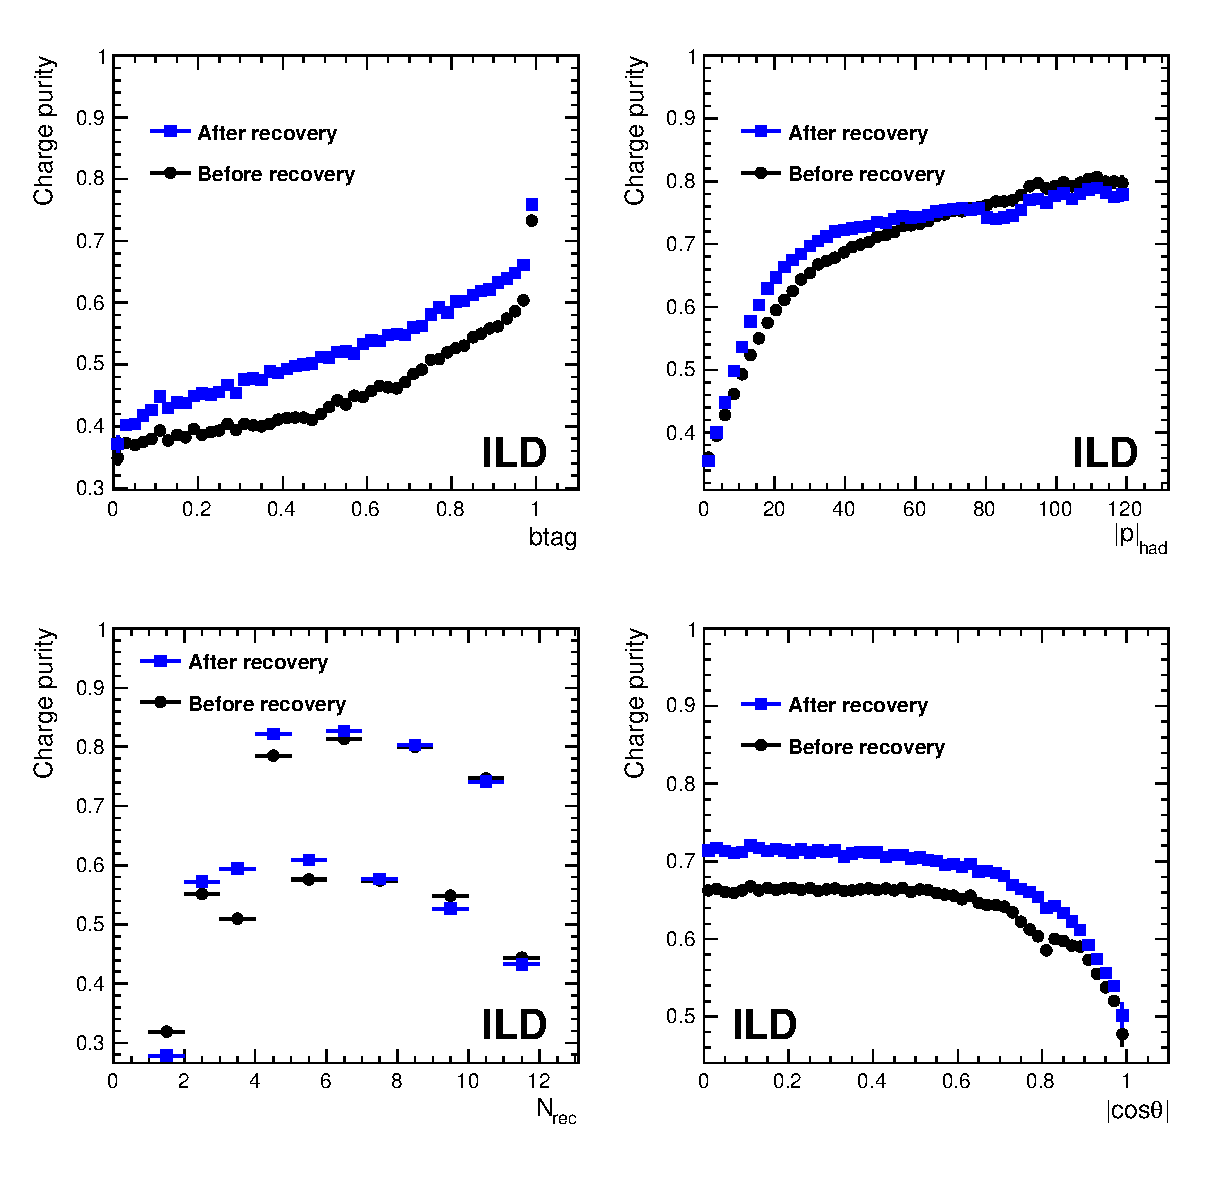
\includegraphics[width=0.8\textwidth]{figures_Methods/b_purity_VR_ttbar_l5.eps}
      \caption{Lower plot, B-quark charge purity in single jets as a function of different kinematic variables, after and before recovery.}
      \label{vr_and_bquarkpurity_ttbar:b}
    \end{subfigure}%
  \end{tabular}
  \caption{$t\bar{t}$.  }
  \label{vr_and_bquarkpurity_ttbar}
\end{figure*}


\begin{figure*}[!ht]
  \centering
  \begin{tabular}{l}
    \begin{subfigure}{\textwidth}
      \centering
      \begin{tabular}{ll}
        \centering
        \includegraphics[width=0.4\textwidth]{figures_Methods/beforeVR_bbbar_l5.eps} & 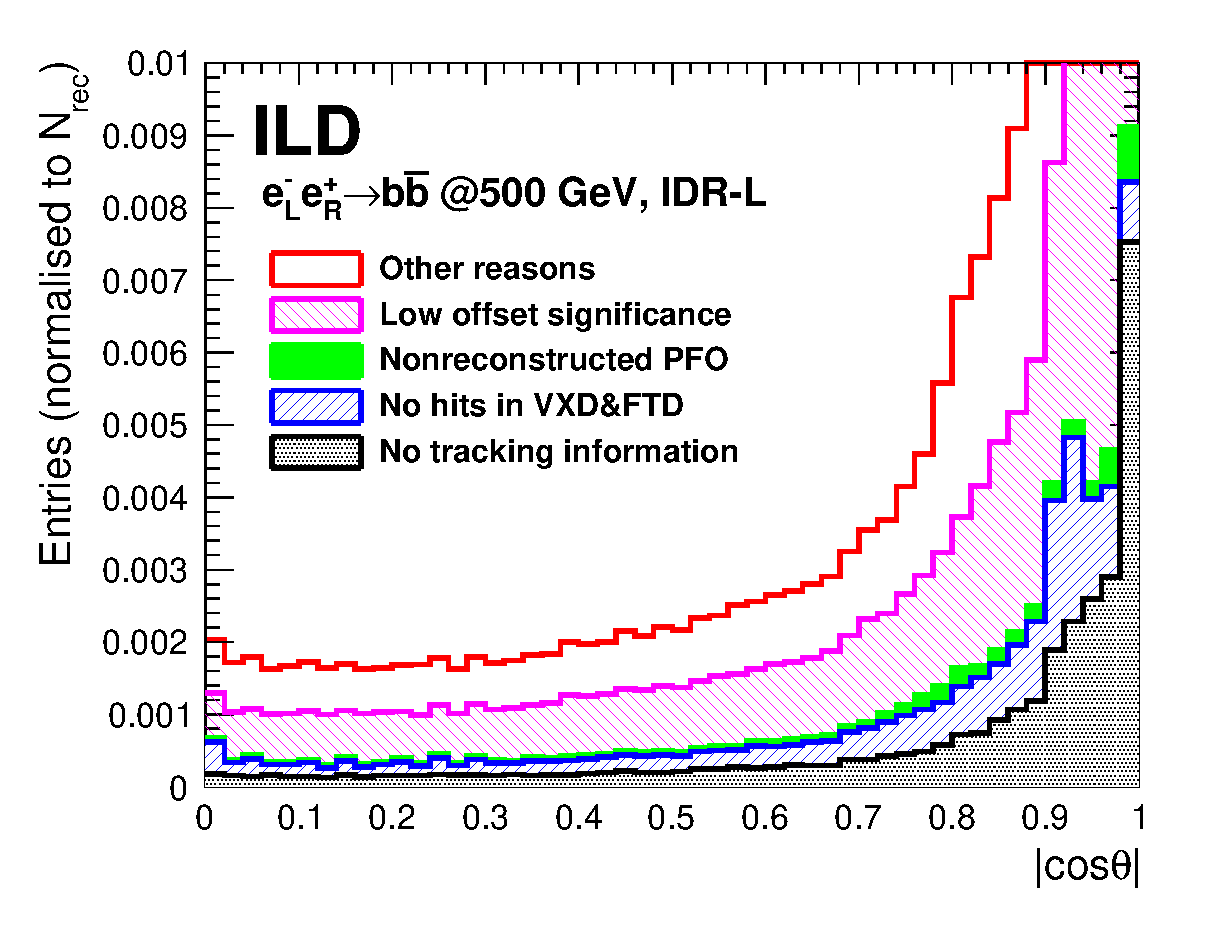
\includegraphics[width=0.4\textwidth]{figures_Methods/afterVR_bbbar_l5.eps}\\
      \end{tabular}
      \caption{ Left, lost tracks in reconstructed vertexes before recovery. Right, lost tracks in reconstructed vertexes after recovery.}
      \label{vr_and_bquarkpurity_bbbar:a}
    \end{subfigure} \\
    \begin{subfigure}{\textwidth}
      \centering
      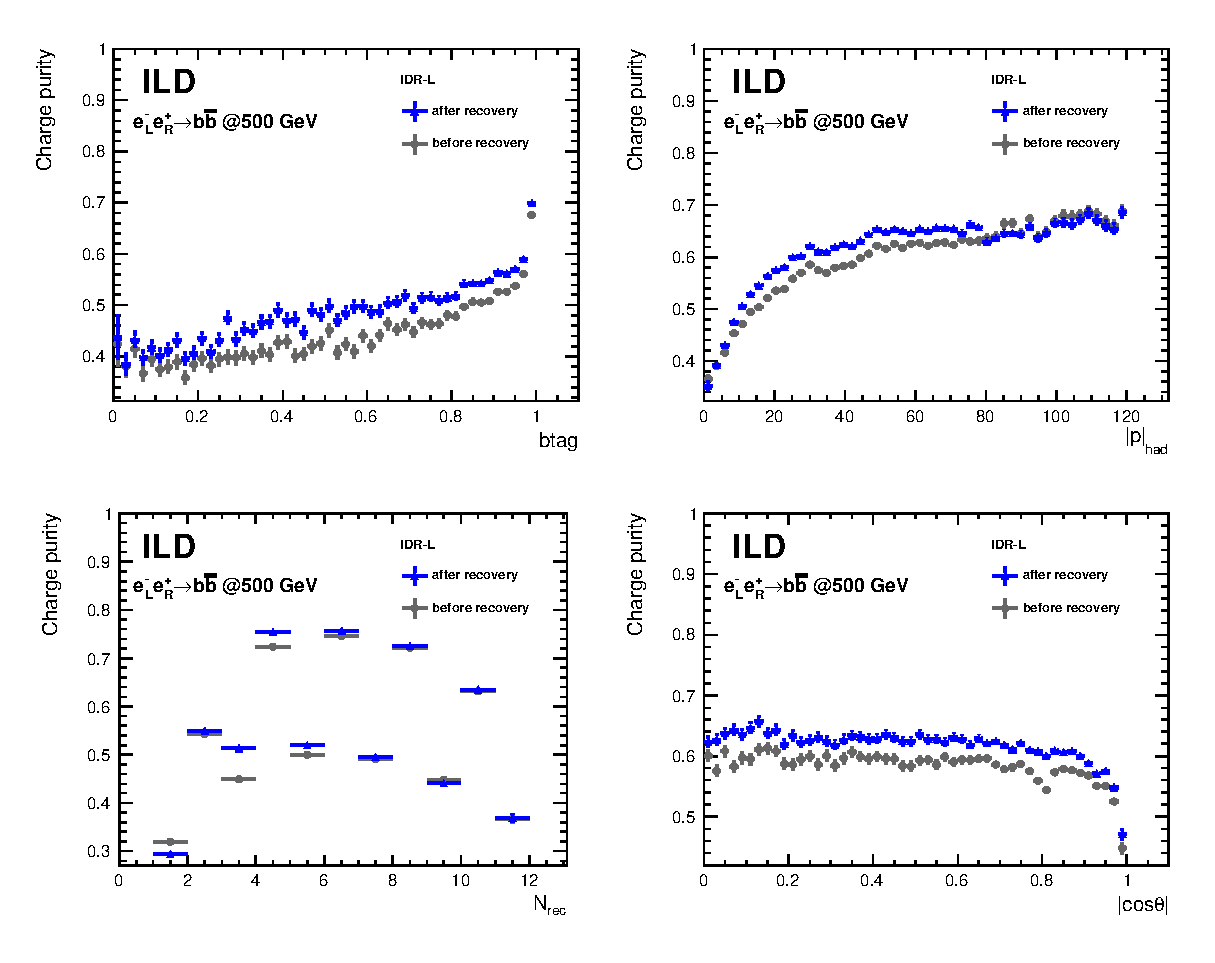
\includegraphics[width=0.8\textwidth]{figures_Methods/b_purity_VR_bbbar_l5.eps}
      \caption{Lower plot, B-quark charge purity in single jets as a function of different kinematic variables, after and before recovery.}
      \label{vr_and_bquarkpurity_bbbar:b}
    \end{subfigure}%
  \end{tabular}
  \caption{$b\bar{b}$.  }
  \label{vr_and_bquarkpurity_bbbar}
\end{figure*}

\begin{figure}[h!]
\centering
  \includegraphics[width=0.8\textwidth]{figures_BBbar/acceptance_2models_v2.eps} 
\caption{Detector acceptance distribution for b-tagged jets.}
\label{fig_acceptance_bb}
\end{figure}

\begin{figure}[h!]
\centering
\begin{tabular}{ll}
  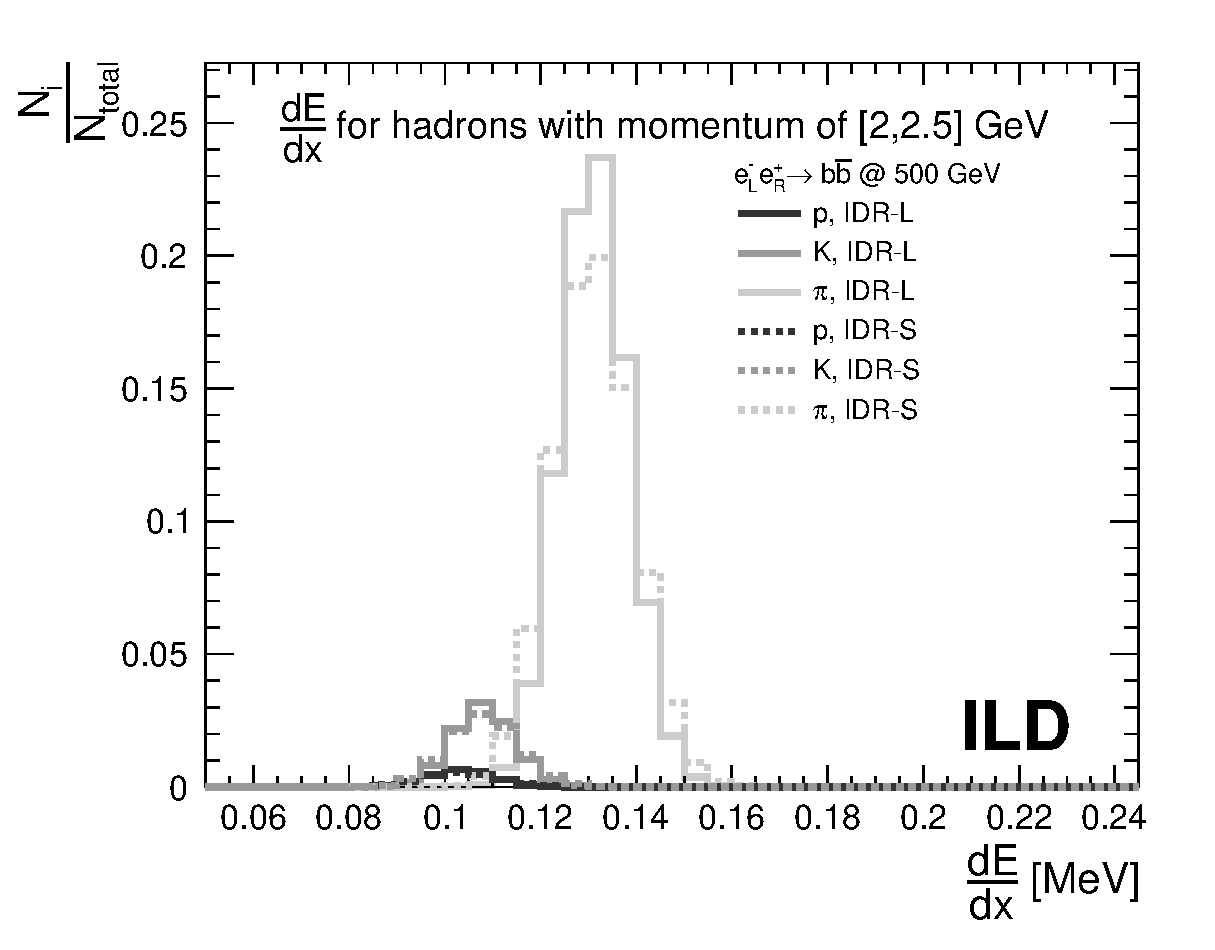
\includegraphics[width=0.5\textwidth]{figures_Methods/separation_had_2GeV_models_v2.eps} & 
  \includegraphics[width=0.5\textwidth]{figures_Methods/separation_had_5GeV_models_v2.eps} \\ 
  \includegraphics[width=0.5\textwidth]{figures_Methods/separation_had_10GeV_models_v2.eps} & 
  \includegraphics[width=0.5\textwidth]{figures_Methods/separation_had_10GeV_models_v2.eps} 	
\end{tabular}
\caption{Projection of dE/dx for several momentum ranges. Comparison of hadron separation performance by different detector models in bbbar final states.}
\label{fig_dEdx_1}
\end{figure}

\begin{figure}[h!]
\centering
\begin{tabular}{ll}
  \includegraphics[width=0.5\textwidth]{figures_Methods/separation_had_2GeV_bbbar_vs_ttbar_v2.eps} & 
  \includegraphics[width=0.5\textwidth]{figures_Methods/separation_had_5GeV_bbbar_vs_ttbar_v2.eps} \\ 
  \includegraphics[width=0.5\textwidth]{figures_Methods/separation_had_10GeV_bbbar_vs_ttbar_v2.eps} & 
  \includegraphics[width=0.5\textwidth]{figures_Methods/separation_had_10GeV_bbbar_vs_ttbar_v2.eps} 	
\end{tabular}
\caption{Projection of dE/dx for several momentum ranges. Comparison of hadron separation performance by the large model for different topologies. }
\label{fig_dEdx_2}
\end{figure}

\begin{figure}[h!]
\centering
  \includegraphics[width=0.8\textwidth]{figures_Methods/kaonIDeff_v2.eps} 
\caption{}
\label{kaonID_effpurity}
\end{figure}

\item Information specific to tt-analysis

\begin{itemize}
\item Energy and polar angle spectrum of selected isolated lepton
\item Table with selection efficiencies
\item For the record we may add the observation by Amjad on the b/c tagging.
\item Purity measurements for double charge selection + efficiencies of different methods.
  \begin{figure}[h!]
    \centering
    \begin{tabular}{ll}
      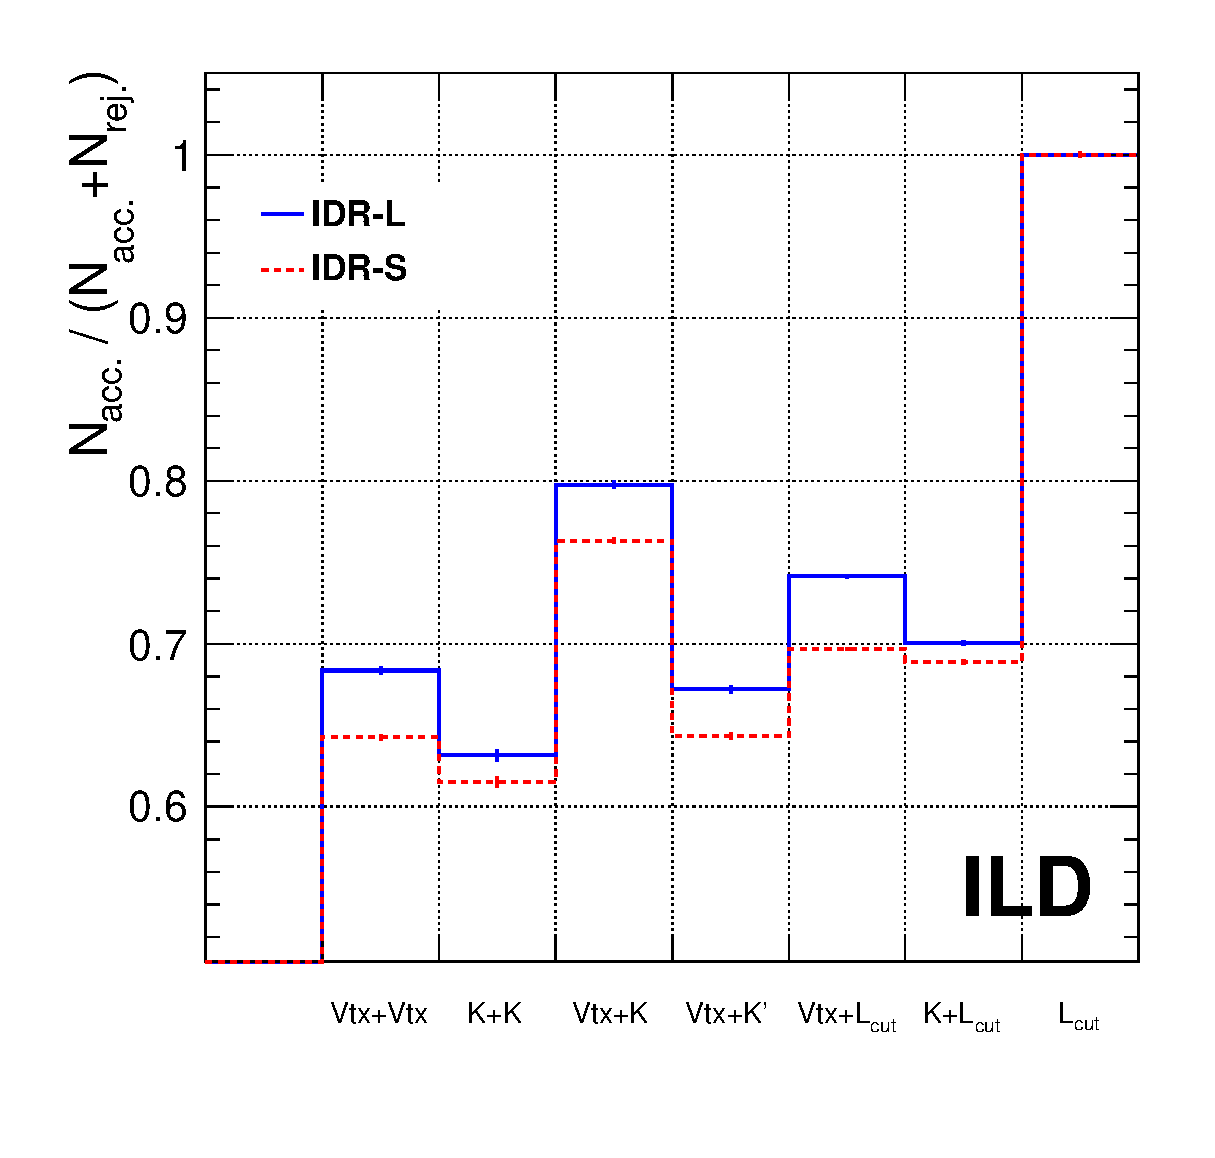
\includegraphics[width=0.5\textwidth]{figures_TTbar/p_value_num_l5_ele_mu.eps} & 
      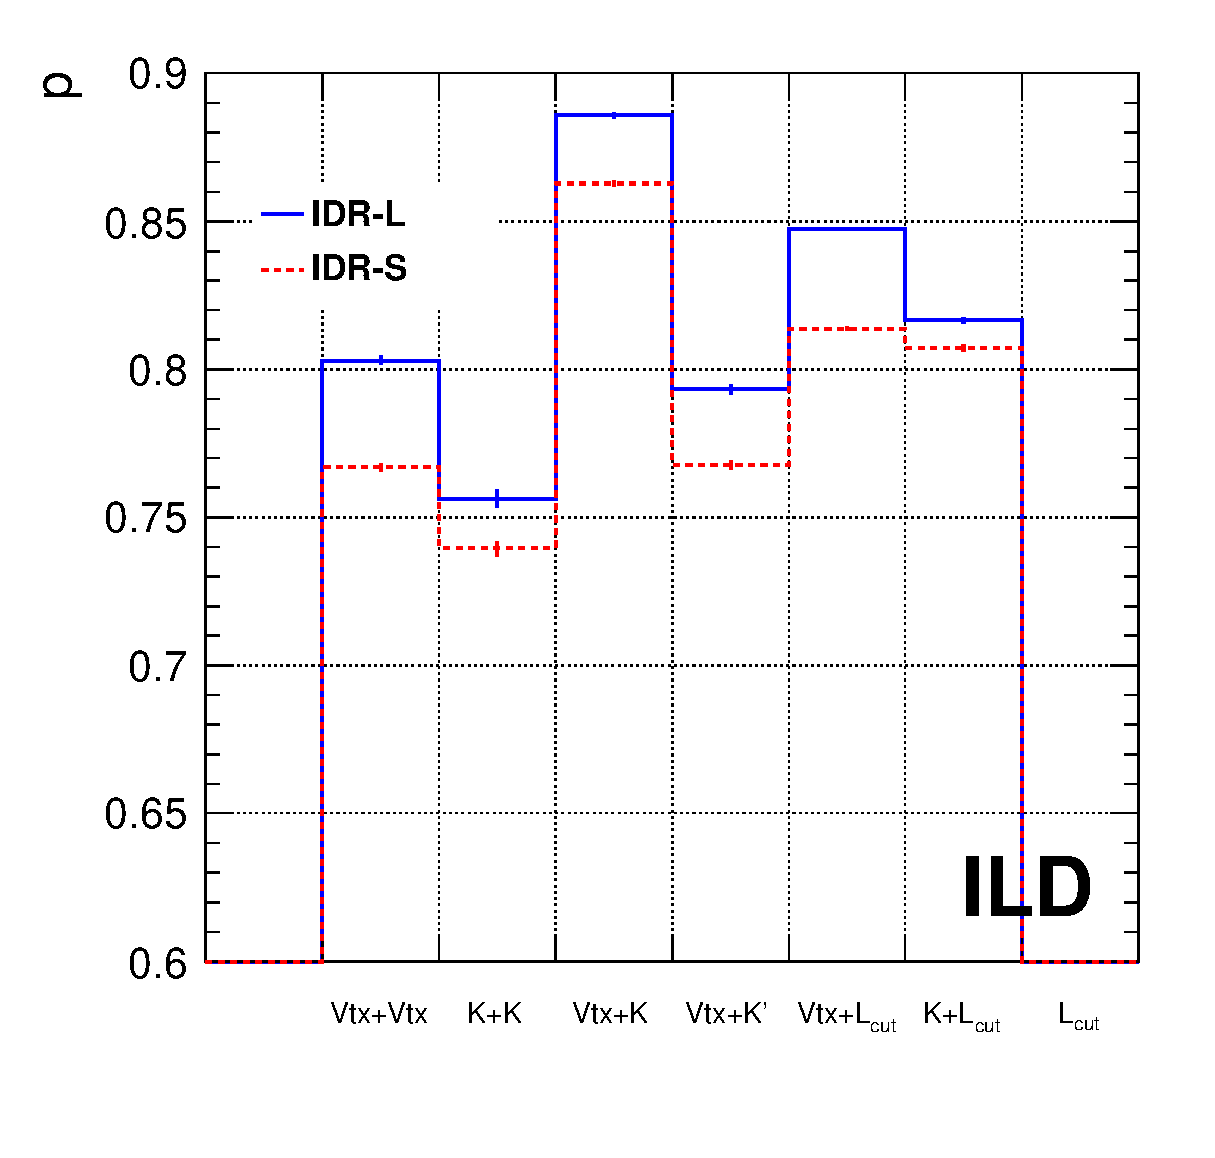
\includegraphics[width=0.5\textwidth]{figures_TTbar/p_value_l5_ele_mu.eps}
    \end{tabular}
    \caption{Calculated probability plots for $t\bar{t}$ events. Left plot shows the result of $N_{acc.} / (N_{acc.} + N_{rej.})$ and right plot shows the p values with different charge configurations.}
    \label{fig_eff_purity}
  \end{figure}
\end{itemize}

\item Information specific to bb analysis
\begin{itemize}
\item Table with selection efficiencies
\item Is there anything specific to the bb analysis given that bb is a subsystem of tt?
\end{itemize}

\begin{table}[t]
  \begin{center}\renewcommand{\arraystretch}{1.6}
    \begin{tabular}{l|l|l|l|l|l|l} 
    \multicolumn{7}{c}{$e_{L}^{-}e_{R}^{+}\rightarrow b\bar{b}$ at 500 GeV }\\
      \hline
      \hline
       & \multicolumn{3}{c|}{IDR-L} & \multicolumn{3}{|c}{IDR-S}\\
       & Signal& B$_{b\bar{b}}$/S & B$_{rad. Z}$/S & Signal & B$_{b\bar{b}}$/S & B$_{rad. Z}$/S\\
      \hline
      Full sample   & 100.0\% & 1800.5\% & 359.1\% & 100.0\% & 1800.6\% & 359.0\% \\
      $b_{tag}(jet_{1})>0.9$ and $b_{tag}(jet_{2})>0.2$    & 70.2\% & 2.3\% & 147.7\%  & 69.9\% & 2.3\% & 149.0\% \\
      $m_{jet_{1}+jet_{2}}>200 GeV$    & 68.2\% & 1.4\% & 6.7\%  & 67.8\% & 1.2\% & 6.7\% \\
      $E_{photon}<100 GeV$    & 64.8\% & 1.3\% & 1.7\% & 64.3\% & 1.2\% & 1.6\% \\
      \hline
      \hline     
    \end{tabular}
 \end{center}
 \label{table_eff_bbbar}
 \caption{Selection efficiency and B/S rejection for some bkg sources}
\end{table}

\begin{table}[t]
  \begin{center}\renewcommand{\arraystretch}{1.6}
    \begin{tabular}{l|l|l} 
    \multicolumn{3}{c}{$e_{L}^{-}e_{R}^{+}\rightarrow b\bar{b}$ at 500 GeV }\\
      \hline
      \hline
       & IDR-L & IDR-S\\
      \hline
      Vtx+Vtx   & 12.9\% & 12.8\% \\
      K+K    & 4.4\% & 4.0\% \\
      Vtx+K (diff. jets)    & 3.9\% & 3.7\% \\
      Vtx+K (same jet) & 7.7\% & 7.4\% \\
      \hline
      \hline     
    \end{tabular}
 \end{center}
 \label{table_charge_calc_bbbar}
 \caption{Final selection efficiency, after double jet-charge measurement}
\end{table}
    
\begin{figure}[h!]
\centering
  \includegraphics[width=0.8\textwidth]{figures_BBbar/purity_v2.eps} 
\caption{Purity of the different methods}
\label{purity_bb}
\end{figure}



\end{itemize}




\subsection{Limits of $ee\rightarrow bb$ at 500\,GeV}

\begin{itemize}
\item Here I wanted to point out why the bb at 500 GeV is more involved than at 250 GeV but given the results shown today by Adrian this is maybe less of an issue.
\end{itemize}

%|||||||||||||||||||Interaction zone|||||||||||||||||||||||

\section{Results}
 
 \begin{figure}[h!]
\centering
  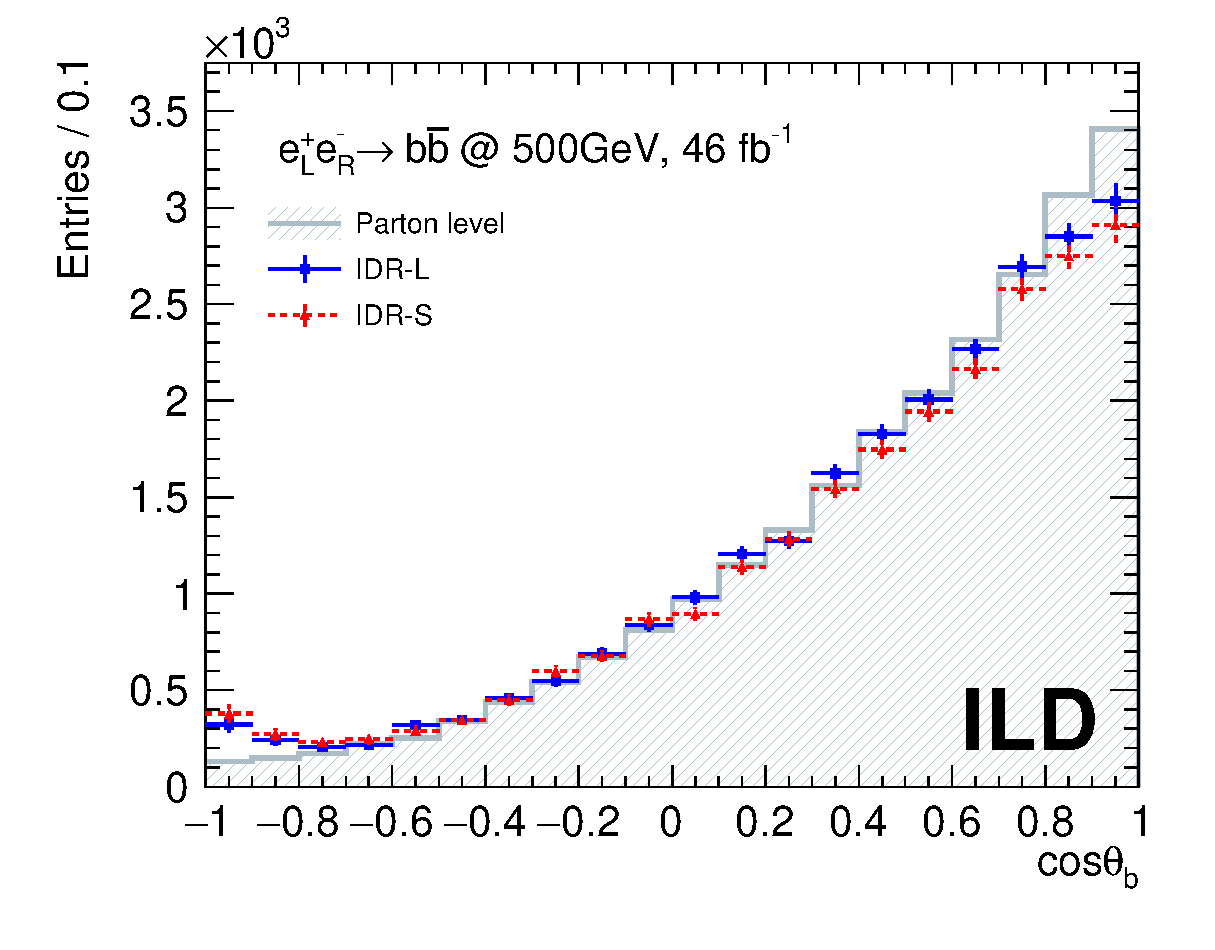
\includegraphics[width=0.8\textwidth]{figures_BBbar/result2models_v2.eps} 
\caption{}
\label{results_bb}
\end{figure}

\begin{itemize}
\item Polar angle spectrum $ee\rightarrow bb$ (Large and small)
\item $ee\rightarrow tt$  including underlying b polar angle spectrum (Large and small)
\end{itemize}




%\begin{figure}[H]
%\centering
%\includegraphics[width=.50\linewidth]{new-ntracks-graph.pdf}
%\caption{\label{fig:fulltrackgraph} \sl The average number of secondary tracks $\left< N_{\mathrm{tracks}} \right>$ as a function of the beam energy. Other details follow those of Fig.~\ref{fig:irgraph}. 
%for data (black points with error shaded band) in comparison to the three simulation models, \qgsp\ (blue squares), \ftfp\ (green upward-pointing triangles) and \qbbc\ (red downward-pointing triangles).  Error bars represent statistical errors and the error band the systematic error from the correction for double $\uppi^-$ background.
%}
%\end{figure}

%|||||||||||||||||||||Hit distribution||||||||||||||||||||||


\section{Summary}

The process $ee\rightarrow tt$ has been successfully ported from the `DBD world' to the `IDR World'. No major differences between short and large detectors. \\

FURTHER SUGGESTIONS ARE WELCOME.


\section*{Acknowledgements}
%Tu peux faire ca avant la migration. 
%{\it [Data-set specific thanks to laboratories, technical staff, non-CALICE institutes providing equipment, ... --- not added now ---  ]}
%We gratefully acknowledge the DESY, CERN and FNAL managements for their support and hospitality, and their accelerator staff for the reliable and efficient beam operation.
%This work was supported 
%by the FWO, Belgium; 
%by the Natural Sciences and Engineering Research Council of Canada;
%by the Ministry of Education, Youth and Sports of the Czech Republic;
%by the European Union's Horizon 2020 Research and Innovation programme under Grant Agreement 654168; %% AIDA-2020
%by the European Commission within Framework Programme 7 Capacities, Grant Agreement 262025;  %% AIDA (not 2020)
by the P2IO LabEx in the framework 'Investissements d'Avenir' managed by the French National Research Agency (ANR) under Grant Agreements ANR-10-LABX-0038 and ANR-11-IDEX-0003-01; 
by the `Quarks and Leptons' Programme of CNRS/IN2P3 France;
by the `Prestige/MSCA Programme;
%by the Alexander von Humboldt Stiftung (AvH), Germany;
%by the Bundesministerium f\"ur Bildung und Forschung (BMBF), Germany; 
%by the Deutsche Forschungsgemeinschaft (DFG), Germany; 
%by the Helmholtz-Gemeinschaft (HGF), Germany; 
%by the I-CORE Program of the Planning and Budgeting Committee, Israel;
%by the Nella and Leon Benoziyo Center for High Energy Physics, Israel;
%by the Israeli Science Foundation, Israel;
%by the National Research Foundation of Korea;
%by the Korea-EU cooperation programme of National Research Foundation of Korea, Grant Agreement 2014K1A3A7A03075053; 
%by the Netherlands Organisation for Scientific Research (NWO);
%by the Science and Technology Facilities Council, UK;
%by the Nuclear Physics, Particle Physics, Astrophysics and Cosmology Initiative, a Laboratory Directed Research and Development program at the Pacific Northwest National Laboratory, USA.
%{\it [add your funding agency here, grant numbers only if absolutely required]}.

%In conclusion, there is no preference for {\sc Geant4} physics lists as none of the two models, used in the analysis, describe the data in high detail. 
%-------------------------------------------------------------------
%-------------------------BIBLIOGRAPHY------------------------------
%-------------------------------------------------------------------
%\begin{thebibliography}{100} 
%\bibitem{bib:Calorimetry} J. C. Brient, H. Videau,\emph{ The calorimetry at the future $e^+e^-$ linear collider}, in: Proceedings of the APS / DPF / DPB Summer Study on the Future of Particle Physics (Snowmass 2001), 2001,arXiv:hep-ex/0202004v1.
%\bibitem{bib:ecal} The CALICE collaboration, \emph{Design and electronics commissioning of the physics prototype of a Si-W electromagnetic calorimeter for the International Linear Collider}, J. Instrum. 3 (2008) P08001, arXiv:0805.4833v1 [physics.ins-det]
%\bibitem{bib:Naomi} The CALICE Collaboration,  \emph{Testing Hadronic Interaction Models using a Highly Granular Silicon-Tungsten Calorimeter}, Nucl. Instrum. Meth. A Volume 794, Pages 240–254, arXiv:1411.7215v2 [physics.ins-det]
%\bibitem{bib:2010_CALICE_2} The CALICE Collaboration, C. Adloff, et al., \emph{Construction and Commissioning  of the CALICE Analog Hadron Calorimeter Prototype}, J. Instrum.~(5)  (2010) P05004, arXiv:1003.2662v1 [physics.ins-det].
%\bibitem{bib:2012_CALICE} The CALICE Collaboration, C. Adloff, et al., \emph{Construction and performance of a silicon photomultiplier/extruded scintillator tail-catcher and muon-tracker}, J. Instrum. (7) (2012) P04015, arXiv:1201.1653 [physics.ins-det].
%\bibitem{bib:G4pl} The {\sc Geant}4 Collaboration, \emph{Reference Physics Lists}, \url{http://Geant4.cern.ch/support/proc_mod_catalog/physics\_lists/referencePL.shtml}
%\bibitem{bib:HLi} \emph{Higgs Recoil Mass and Cross-Section Analysis at ILC And Calibration of the CALICE SiW ECAL Prototype}, Ph.D. thesis, Universit\'e Paris Sud   - Paris XI (2012).
%\bibitem{bib:2012_Doublet} P.Doublet, \emph{Hadrons dans un calorim\`etre \'electromagn\'etique   silicium-tungst\`ene hautement granulaire -- Production du quark top \'a   l'International Linear Collider}, Ph.D. thesis, Universit\'e Paris Sud   - Paris XI (2012).
%\end{thebibliography}
\section*{References}
\begin{footnotesize}
%
%\bibliographystyle{utphys_mod}
%\bibliography{had-pap}
%
%\bibliographystyle{hep}

%\renewcommand\refname{References}
%\end{thebibliography}
\end{footnotesize}


%The following plots in Fig. \ref{fig:rtotexample} and \ref{fig:rtotalrgraph} allow to establish a connection between Ref. \cite{bib:Naomi} and the present study. Regarding the difference in units of measurement and different selection by interaction layer, the Fig. \ref{fig:rtotalrgraph} is similar to its analogue in Ref. \cite{bib:Naomi}.
%\begin{figure}[H]
%\centering
%\begin{subfigure}{0.5\textwidth}
%\centering
%\includegraphics[width=.90\linewidth]{stdselection/r-total-2.pdf}
%\caption{\label{fig:rtot2} 2\,GeV primary particle.}
%\end{subfigure}% 
%\begin{subfigure}{0.5\textwidth}
%\centering
%\includegraphics[width=.90\linewidth]{stdselection/r-total-10.pdf}
%\caption{\label{fig:rtot10} 10\,GeV primary particle.}
%\end{subfigure}
%\caption{\label{fig:rtotexample} A comparison of mean radius of event hits between Monte Carlo samples and data with 2 (left) and 10 (right) GeV beam energy. The histograms are normalized to unity in order to compare samples with different event number. Error bars on the plot represent statistical uncertainties only.}
%\end{figure}

%\begin{figure}[H]
%\centering
%\includegraphics[width=0.5\textwidth]{stdselection/r-total-graph.pdf}
%\caption{\label{fig:rtotalrgraph} A mean radius of hits in the \ecal\ for data and various Monte Carlo physics lists as a function of beam energy (2\,GeV to 10\,GeV). Error regions on the graph represent statistical uncertainties only.}
%\end{figure}

%\begin{figure}[H]
%\centering
%\includegraphics[width=0.5\textwidth]{stdselection/combination.pdf}
%\caption{\label{fig:epsilondatasys} Mean number of tracks found by the \tfa\ with different \ep\ values for 2, 4, 6, 8 and 10\,GeV beam energy of the \qgsp\ simulation and data. The difference between data and corresponding simulation curves is caused by an underestimation of number of clusters by the physics list model. The saturation value of $<N_{tracks}>$ is gradually increasing with the beam energy. }
%\end{figure}

\clearpage

%%%%%%%%%%%%%% 

\section*{Analysis of $e^+e^-\rightarrow t\bar{t}$}

\begin{itemize}

\item Settings
  \begin{itemize}
  \item ILCSoft v02-00-02
  \item Used yyxylv and yyxyev events (eliminated isolated tau)
  \item Polarization of eLpR is used.
  \end{itemize}
  
\item Polar angle distribution of $t\bar{t}$
  \begin{itemize}
  \item Full statistic polar angle
  \item Polar angle distribution of $t\bar{t}$ of the generated and reconstructed data. Red dotted line shows the fitted result of the reconstructed events.
  \item $t\bar{t}$ polar angle for large (l5) and small (s5) models. (Figure.~\ref{compare})
      
  \begin{figure}[h!]
    \centering
    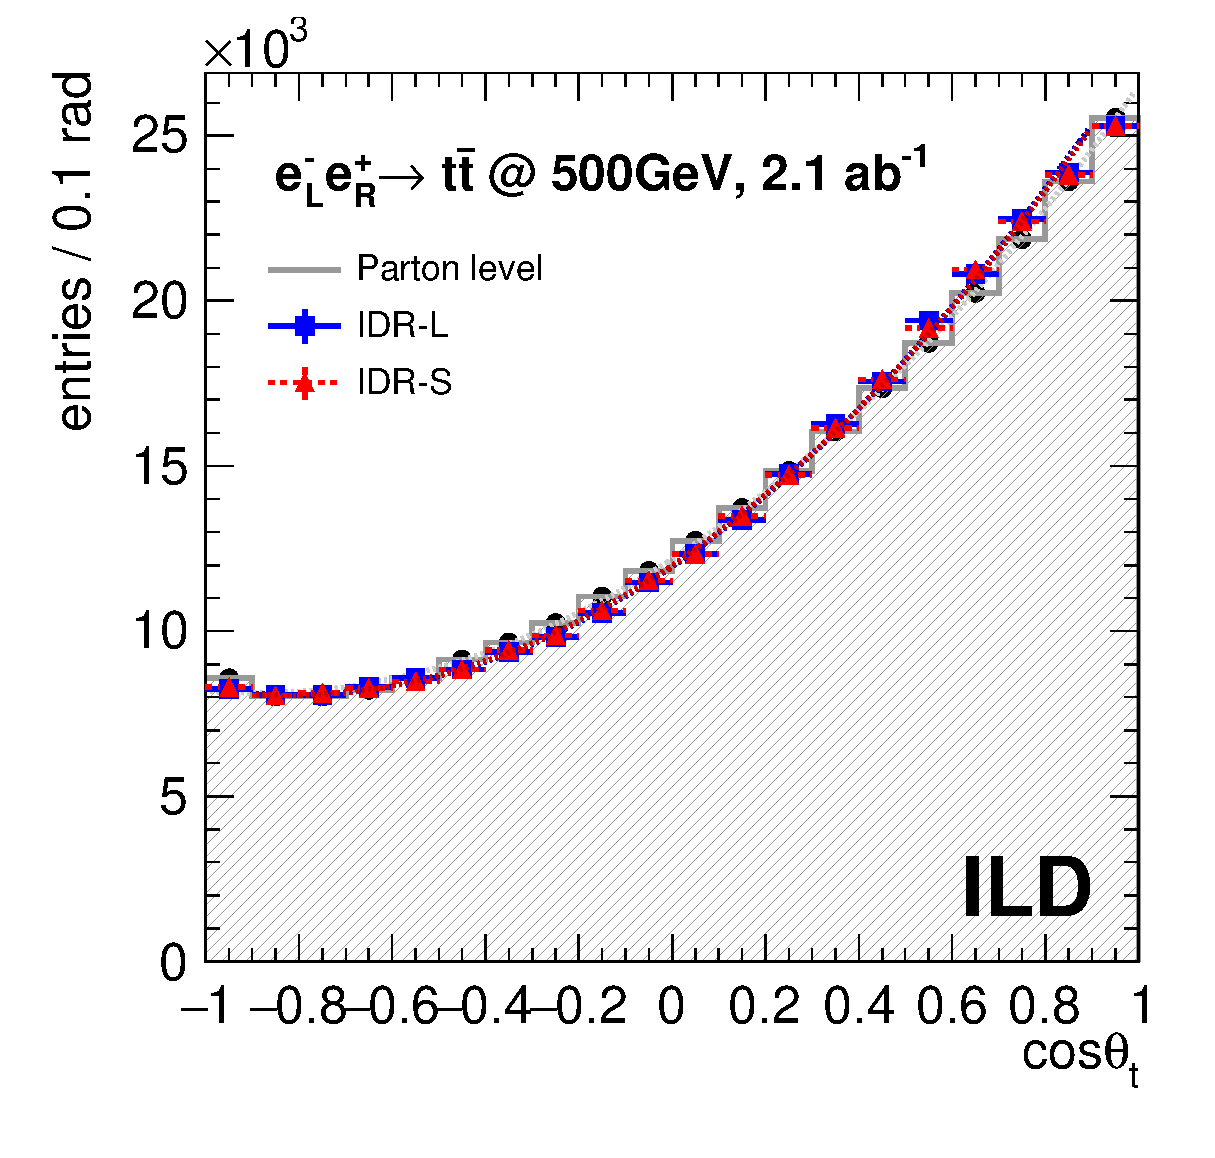
\includegraphics[width=0.5\textwidth]{figures_TTbar/results2models_t.eps} 
    \caption{Polar angle distribution for top quark. Distributions for IDR-S is normalized to the one for IDR-L so that both histograms will be on the same level. }
    \label{compare}
  \end{figure}

    \item Final efficiencies
    
  \begin{table}[h!]
    \parbox{.45\linewidth}{
    \centering
    \begin{tabular}{ccc}
      \hline
      \hline
      	Afb gen				&	0.328685		&	N: 1812768	\\
      	Afb reco			&	0.341900		&	N: 277435		\\
      	Final efficiency	&	30.609\%		&						\\		
      \hline
      \hline
    \end{tabular}
    \caption{l5 final efficiency and $A_{fb}$}
    }
    \hfill
    \parbox{.45\linewidth}{
    \centering
    \begin{tabular}{ccc}
      \hline
      \hline
      	Afb gen				&	0.328848		&	N: 1866364	\\
      	Afb reco			&	0.340474		&	N: 284183		\\
      	Final efficiency	&	30.4531\%	&						\\		
      \hline
      \hline
  \end{tabular}
  \caption{s5 final efficiency and $A_{fb}$}
  }
  \end{table}
  
  \item No significant differences were confirmed between s5 and l5 samples. For the $t\bar{t}$ studies, we see that the polar angle distribution is consistent with the Parton level result. At the edges of the polar angles, we do not see inefficiencies due to the detector geometry. Inefficiencies of at the edges of the detectors originates from inability to reconstruct b jets going to the forward region. For the top pair reconstruction, we can also rely on W informations thus not losing much efficiencies at the edges.



\break

  

\end{itemize}

  
  \item Polar angle distribution of $b\bar{b}$
  \begin{itemize}
  \item Full statistic polar angle
  \item We could put each figures side by side for comparison. For example, we can put $t\bar{t}$ and $b\bar{b}$ plots side by side with same detector model.
  \item $b\bar{b}$ polar angle for large (l5) and small (s5) models (Figure.~\ref{compare_b})
  
%    \begin{figure}[h!]
%      \centering
%        \begin{tabular}{ll}
%          \includegraphics[width=0.5\textwidth]{figures_TTbar/b_polar_l5_ele_mu.eps} & 
%          \includegraphics[width=0.5\textwidth]{figures_TTbar/b_polar_s5_ele_mu.eps}
%        \end{tabular}
%        \caption{Left is l5 and right is s5}
%        \label{fig_polar_ttbar}
%    \end{figure}

     \begin{figure}[h!]
        \centering
        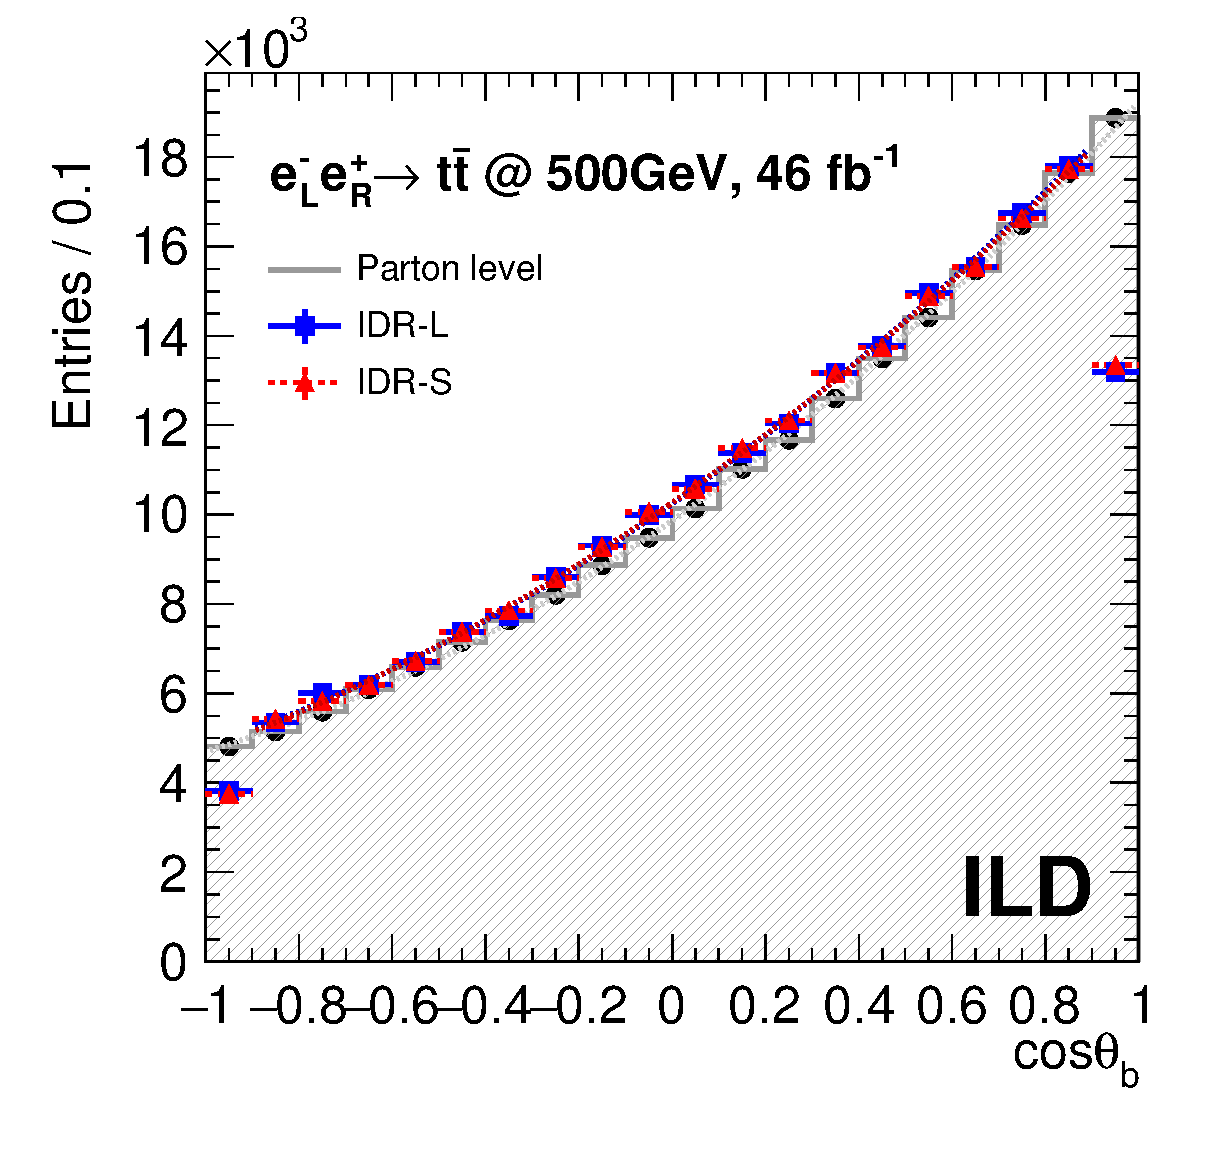
\includegraphics[width=0.5\textwidth]{figures_TTbar/results2models_b.eps} 
        \caption{Hadronic polar angle distribution. Distributions for IDR-S is normalized to the one for IDR-L so that both histograms will be on the same level.}
        \label{compare_b}
    \end{figure}

  
  \end{itemize}
  
  
  \break
  

  \item Others
      
    \begin{figure}[h!]
      \centering
        \begin{tabular}{ll}
          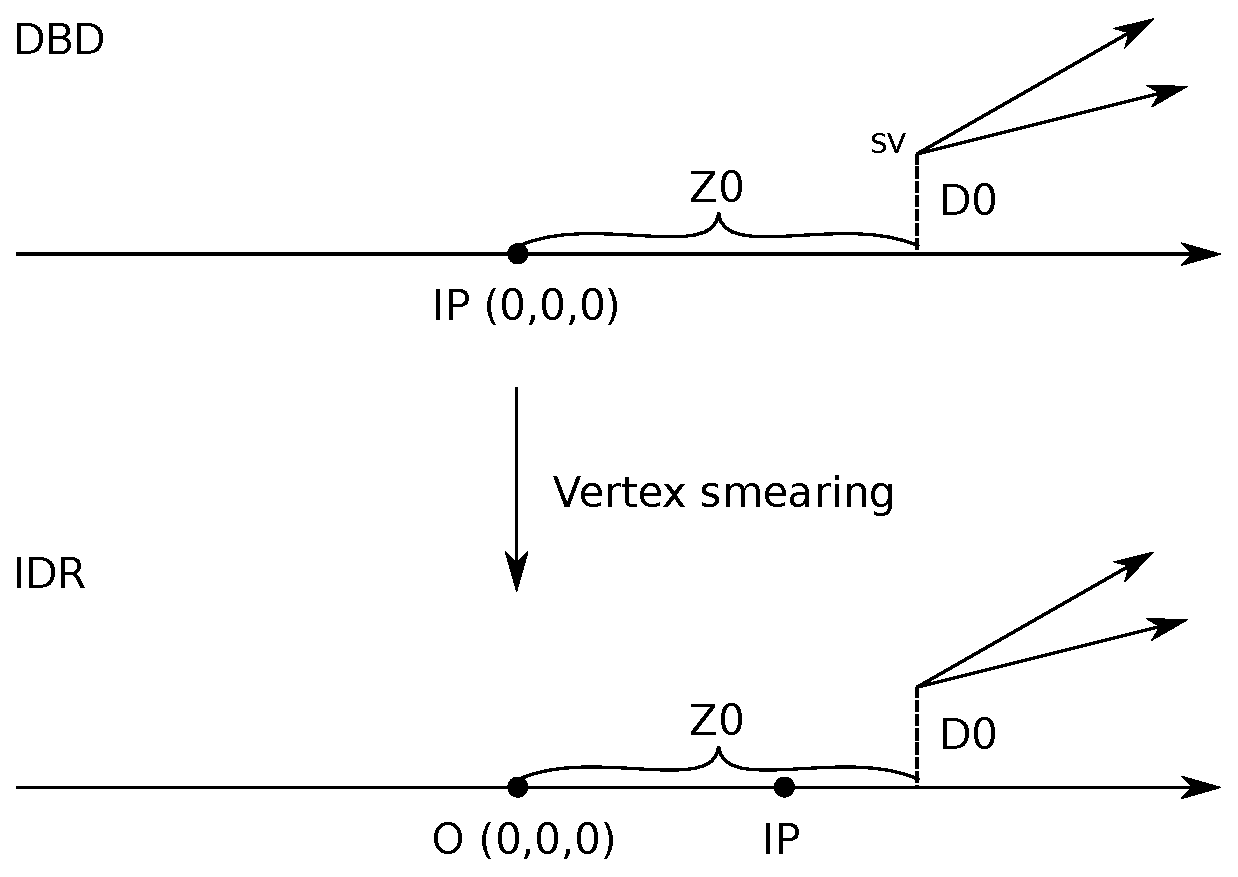
\includegraphics[width=0.5\textwidth]{figures_Methods/drawing.eps} & 
          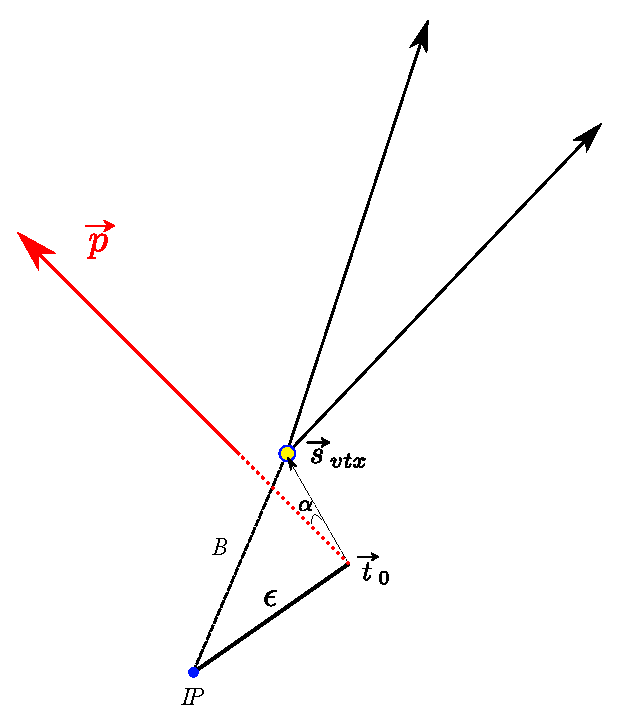
\includegraphics[width=0.5\textwidth]{figures_Methods/vertex_recovery.eps}
        \end{tabular}
        \caption{Left is }
        \label{fig_vtx_restore_schematics}
    \end{figure}
          
  
\end{itemize}



























\end{document}
